\newpage
\part{The Model}

The Proportional Hazards Model is one of the most used statistical techniques in the world. It was introduced by Cox \fcite{cox1972regression} with the aim of extending the results of Kaplan and Meier \fcite{kaplanmeier} "to the comparison of life tables and more generally to the incorporation of regression-like arguments into life-table analysis." Interestingly, these two papers are two of the most cited papers in statistics according to Ryan and Woodall \fcite{ryanwoodall}. So why is the Cox model so popular?

The Cox model is very attractive to statisticians because it is semi-parametric. What this effectively means is the hazard is divided into two parts:

\begin{itemize}
    \item a baseline hazard (which can be entirely arbitrary, nonparametric and time-dependent) which is common across all subjects, and
    \item a relative risk parameter which describes the effects of covariates on the hazard.
\end{itemize} 

This separation allows statisticians to build models based on the covariates without explicit or iterative calculation of the baseline hazard.

In this part of the thesis, I will describe the model in detail as proposed by Cox and explore surrounding methods and extensions. In section \ref{background}, I will give a history of the statistics used by Cox in the development of the model and the assumptions it is based upon. \Cref{sec:partial-likelihood} will consider the partial likelihood function as discussed in Cox \fcite{cox75}, why it can be consider it a full likelihood and why this is of benefit. Some methods of approximating and extending the original partial likelihood introduced by Cox \fcite{cox1972regression} (which dealt solely with continuous time events) will be introduced briefly. Section \ref{baseline} will deal with the motives and methods for estimation of the baseline hazard.

\section{Background}\label{background}

The Cox model implements the hazard function in terms of a baseline hazard and a function of the covariates as follows

\begin{equation}\label{cox-hazard}
    \lambda(t;\z)=\lambda_0(t)e^{(\z\Beta)}.
\end{equation}

It is preferred over the logistic model for estimating survival time distributions as it considers the censored data and thus can obtain more information. The general approach to solving the model would first estimate the regression coefficients, then choose or estimate a suitable distribution for the baseline hazard, and finally estimate the full survivor and hazard functions.

The Cox model has two primary uses: variable impact estimation and survival time estimation. Of course, they impact one another but they are distinct.

Covariate impact can be estimated using model selection for the Cox model, this is the main focus of this thesis and is discussed in depth in part II. By estimating the regression coefficients to give the best model possible, the extent to which each covariate impacts the model is predicted. This hopefully allows for interpretable results which are useful in many fields for discovering: impactful genomes in cancer epidemiology, impact of material density on machine part failure, impact of age on loan defaulting, et cetera. 

Survival time or time-to-event estimation can be useful for predicting how long a patient is expected to live after a given diagnosis or the probability that a subject will default on their loan before repayment. The distributions underlying these regression estimations are of huge importance in medical, actuarial, business and engineering studies.

\subsection{Censoring}

I introduced censoring in section \ref{intro-censoring} and explained that most of the censoring that will be dealt with is right censoring. Here I would like to give a brief insight into how right censoring is usually dealt with and how it can affect the results of the model.

Obviously, it is beneficial to include as much information can be from the data when building the model. Thus in normal procedure, the individuals are included up until the point at which they are censored, then are removed from calculation at the end of the interval in which they are censored. 

Think of this as follows: if there is a set of $\{1,2,3,4\}$ of individuals and is is observed that 1 fails first, then 2 is censored, 3 then fails and finally 4 fails, the probability that at the time of first failure 1 fails as observed is given by $$pr(1\textrm{ fails}|\textrm{there is one failure from }\{1,2,3,4\})=\frac{pr(1)}{pr(1)+pr(2)+pr(3)+pr(4)}.$$ Individual 2 is then censored and the probability that 3 fails next is given by $$pr(3\textrm{ fails}|\textrm{there is one failure from }\{3,4\})=\frac{pr(3)}{pr(3)+pr(4)}.$$

In the commonly used methods, increased censoring will lead to an increase in bias in the model, i.e. in our example above, if subjects 2 and 4 were censored in the interval between failure of 1 and 3, the probability of 3 failing would be increased thus giving it more weight in the likelihood estimations introduced below in section \cref{sec:partial-likelihood}.

Robins et al \fcite{robins-rotnitzky-92, robins-93, robins-finkelstein-00} discuss methods to deal censoring to produce consistent and asymptotically normal parameter estimation in the presence of censoring. The approach taken is to assume that given survival to a certain time $t_{(i)}$ and the covariate values $\z_{(i)}$, the censoring the in following interval is independent of survival time. This is referred to as  missing at random (MAR). However these methods are not commonly used and in the usual process as it is not always certain that the data is MAR.

Other possibilities are missing completely at random (MCAR) in which missingness / censoring occurs entirely at random, i.e. independently of the covariates and unknown parameters. Cox \fcite{cox1972regression} stated this was an unsatisfactory assumption and should not be used. The last type of missing data which is relatively common is missing not at random (MNAR) in which data is assumed to be missing or censored due to some condition or a dependence on covariates. E.g. in a depression study where patients are more likely to stop checking in if they become more depressed.

\subsection{Proportional Hazards}

The assumption of proportional hazards is the basis of the model introduced by Cox \fcite{cox1972regression}. If we have $n$ independent and identically distributed variables $T_i$ which have the hazard distribution defined by the Cox model, it is assumed that the hazard of one individual is proportional to the hazard of any other individual.

It can easily be seen that every hazard function is proportional to the baseline hazard under the assumption by rearranging \bref{cox-hazard} to give

\begin{equation}\label{prop-hazard}
    \frac{\lambda(t;\z)}{\lambda_0(t)}=\exp(\z\Beta).
\end{equation}

Clearly, the right side is not a function of $t$ and so the both sides are time invariant. The proportional hazards assumption holds if \bref{prop-hazard} holds. This condition can be restated as

\begin{equation}
    \Beta_\xi(t) = c\space \forall \xi\in\{1,\ldots,p\},
\end{equation}

i.e. the coefficients are time-invariant and have a scaling effect on the baseline hazard. Consider as well the hazard function for two subjects $j$ and $j'$ defined as in \bref{cox-hazard}. Dividing one by the other to find the proportion gives

\begin{equation}\label{hazard-ratio}
    \frac{\lambda(t;\z_j)}{\lambda(t;\z_{j'})} =\frac{\lambda_0(t)\exp(\z_j\Beta)}{\lambda_0(t)\exp(\z_{j'}\Beta)}=\frac{\exp(\z_j\Beta)}{\exp(\z_{j'}\Beta)}=e^{(\z_j-\z_{j'})\Beta},
\end{equation}

which is clearly time invariant on the right side and so must be time invariant on the left side as well. In layman's terms, this means if a subject 1 is twice as likely to have an event as subject 2, then this hazard ratio is constant, irrespective of time.

There are extensions of the Cox model discussed by Cox \fcite{cox1972regression} to remove the proportional hazards assumption. These extensions allow for time-dependent covariates and time-dependent coefficients to be considered (see section \ref{extensions}). The extensions to the Cox model normally involve using splines or fractional polynomials, however it has been suggested in some model comparison discussions, see Patel et al \fcite{compphaft}, that more consideration be given to other hazard structures, namely the AFT. Rubio et al \fcite{rubioetal} explores the various hazard structures mentioned in the introduction and concludes that the AIC is a suitable method for selecting the hazard structure.

\subsubsection{Testing Proportional Hazards}

Equation \bref{hazard-ratio} is referred to as the hazard ratio and as mentioned is constant over time. We are able to test that all hazard ratios within the model are constant with time using both goodness-of-fit testing and graphical methods.

The essence of testing for proportional hazards boils down to examination of the coefficients. The null hypothesis states that the coefficients are time-invariant; should a test of the time-dependency of the coefficients give a statistically significant result that points to the rejection of the null hypothesis, the proportional hazards assumption has been broken and one of either an ad hoc modification, an extension to the model or a different model must be used.

There are many different graphical analysis methods to determine if the proportional hazards methods are likely to hold. Hess \fcite{hess95} suggests eight methods of graphical analysis, five of which are compared by Perrson \fcite{persson07} with the method proposed by Arjas \fcite{arjas88} in a simulation study using a Kolmogorov-Smirnov like maximum deviation criterion. Perrson \fcite{persson07} concludes that the Arjas plot is generally the preferred technique if the form of the hazard is anything but increasing, in which case either a smoothed plot of scaled Schoenfeld Residuals versus time or a smoothed plot of the ratio of log cumulative baseline hazard rates versus time are recommended.

Despite the advantages of the aforementioned tests, one of the most commonly used methods is using Kaplan-Meier plots. The data is stratified and the K-M curves are plotted. The curves should be proportional, i.e. they should not cross nor diverge.  

Graphical analysis can prove useful but it is limited in that it is difficult to define objective rules as to what would be deemed to reject the proportional assumptions hypothesis. Most of these methods also will not work well with continuous covariates as the graphs become too cluttered.

The most common methods used for testing proportional hazards in statistical software are residuals, including:

\begin{itemize}
\begin{spacing}{0}
    \item Cox-Snell Residuals
    \item Martingale Residuals
    \item Deviance Residuals
    \item Schoenfeld Residuals
    \item Scaled Schoenfeld Residuals
\end{spacing}
\end{itemize}

I will not discuss in more detail here how these residuals work; for details on how they are used within statistical software in relation to the Cox Model see Hintze \fcite{hintze2007user}.

It is worth mentioning the disadvantages of carrying out tests regarding proportional hazards. Of course it can be useful to check our assumptions hold, but we must now also consider the error implicit in the preliminary test carried out. It is possible that we get a false result for our appropriate model test. If we get a false positive, we could be using the Cox PH model when the hazards are indeed not proportional, or a false negative could lead to rejection of the Cox PH model when it accurately describes the data distribution.

\section{Partial Likelihood}\label{sec:partial-likelihood}

A likelihood function is used to measure the goodness of fit of a statistical model based on a given set of data when the parameters of the model are unknown. It is a function of the parameters only and thus treats the random variables in the dataset as though they were fixed.

It is often the aim to maximise the likelihood function so that we find the parameters which will best fit the model. This parameter vector which maximises the likelihood function is referred to as the maximum likelihood estimate (MLE). When computing the MLE, it is often convenient to use the log-likelihood function to convert the difficult to work with products into more friendly summations.

The Bayesian and frequentist frameworks for statistics will be discussed in more detail in part II of this thesis, but it is worth mentioning now that the likelihood function plays a fundamental role in both. In Bayesian statistics, the maximum likelihood estimate is a special case of a maximum a posteriori estimation (MAP) in which the parameters follow a uniform prior distribution. From a frequentist standpoint, the MLE is a special case of an extremum estimator in which the objective function is the likelihood function.

Cox \fcite{cox1972regression} introduced what he misleadingly referred to as a conditional likelihood which was a likelihood function for inference about $\Beta$ conditioned on the set ${t_i}$ of instants at which failure occurs. The logic here is no information about the hazard is contributed at any point other than those times at which failure occurs. 

\subsection{Continuous Time}

I will first consider the case of continuous time ($m_{(i)}=1\forall i$) as Cox \fcite{cox1972regression} did. Extensions to discrete time will be discussed below. For each failure at time $t_i$, the probability that the failure which occurs is the one observed is 

\begin{equation}
    \frac{\lambda(t_{(i)}; \z_i)dt}{\sum_{j\in\R_i}\lambda(t_{(i)}; \z_{j})dt} = 
    \frac{\lambda_0(t_{(i)})e^{\z_i\Beta}}{\sum_{j\in\R_i}\lambda_0(t_{(i)})e^{\z_j\Beta}} = \frac{e^{\z_i\Beta}}{\sum_{j\in\R_i}e^{\z_j\Beta}}.
\end{equation}

This is the ratio of the hazard of the individual on which failure was observed over the sum of hazards across all the individuals who are at risk at time $t_i$. Notice that the baseline hazard cancels out leaving an equation which only varies with $\Beta$. The likelihood function is then:

\begin{equation}\label{partial-likelihood-eqn}
    L(\Beta;\x) = \prod_{i=1}^k \frac{e^{\z_i\Beta}}{\sum_{j\in\R_i}e^{\z_j\Beta}}
\end{equation}

The log-likelihood function for the model conditioned on ${t_i}$ is then given by taking the natural logarithm of the above function and summing over all events as follows:

\begin{align}
    l(\Beta;\x) &= \sum_{i=1}^k \log\bigg(\frac{e^{\z_i\Beta}}{\sum_{j\in\R_i}e^{\z_j\Beta}}\bigg)\\
    &= \sum_{i=1}^k \bigg( \log(e^{\z_i\Beta}) - \log(\sum_{j\in\R_i}e^{\z_j\Beta})\bigg)\\
    &= \sum_{i=1}^k \z_i\Beta - \sum_{i=1}^k \log(\sum_{j\in\R_i}e^{\z_j\Beta})
\end{align}

The above likelihood given by \bref{partial-likelihood-eqn} and the consequent log-likelihood are referred to as a partial likelihood. Cox \fcite{cox75} explained and discussed the partial likelihood. The principle of the partial likelihood is separating, as far as is possible, the incidental parameters and the nuisance parameters as shown by:

\begin{equation}
    L(\theta,\Beta;data) = L(\theta;data)\cdot L(\Beta;data)
\end{equation}

In the case of the Cox PH model, the coefficient vector, $\Beta$, is generally considered the incidental parameters and the nuisance parameter is the baseline hazard, $\lambda_0(t)$.

Consider the data as falling into two categories: right-censored and failure. Individuals observed to fail at time $t_i$ contribute to the density term $f(t_{(i)})$ and individuals censored at $t_i$ contribute to the survivor function $\F(t_{(i)})$. This gives the full likelihood function as

\begin{equation}
    L(\Beta,\lambda_0(\cdot);\x)=\prod_{i=1}^kf(t_{(i)};\Beta)^{\delta_i}\F(t_{(i)};\Beta)^{1-\delta_i}.
\end{equation}

The definition of the hazard function \bref{hazard-function} gives 

\begin{equation}
    L(\Beta,\lambda_0(\cdot);\x)=\prod_{i=1}^k\lambda(t_{(i)};\Beta)^{\delta_i}\F(t_{(i)};\Beta).    
\end{equation}

Substituting for the definition of the survivor function,

\begin{equation}
    \F(t;\Beta)=(\F_0(t))^{\exp(w\Beta)}=\big(e^{-\int_0^t\lambda_0(u)du}\big)^{\exp(w\Beta)},
\end{equation}

allows the likelihood to be written as

\begin{equation}
    L(\Beta,\lambda_0(\cdot);\x)=\prod_{i=1}^k\big(\lambda_0(t_{(i)})e^{w_i\Beta}\big)^{\delta_i}\big(e^{-\int_0^t\lambda_0(u)du}\big)^{\exp(w_i\Beta)}.
\end{equation}

Taking the log of the above likelihood will give the log-likelihood you first stated. Now multiplying by $\bigg(\frac{\sum_{j\in\mathscr{R}_i}\lambda_0(t_{(i)})\exp({w_j\Beta})}{\sum_{j\in\mathscr{R}_i}\lambda_0(t_{(i)})\exp({w_j\Beta})}\bigg)^{\delta_i}$ and cancelling the baseline hazards gives

\begin{equation}
    L(\Beta,\lambda_0(\cdot);\x)=\prod_{i=1}^k\bigg(\frac{e^{w_i\Beta}}{\sum_{j\in\mathscr{R}_i}e^{w_j\Beta}}\bigg)^{\delta_i}\prod_{i=1}^k\big(\sum_{j\in\mathscr{R}_i}\lambda_0(t_{(i)})e^{w_j\Beta}\big)^{\delta_i}\big(e^{-\int_0^t\lambda_0(u)du}\big)^{\exp(w_i\Beta)}.
\end{equation}

Cox \fcite{cox1972regression} argued that the first term here provides most of the information about $\Beta$ and the last two terms contain most of the information about $\lambda_0(\cdot)$. With this in mind, the first term can be treated as a full likelihood when inference about $\Beta$ is the aim. Thus maximising \bref{partial-likelihood-eqn} gives the maximum partial likelihood estimate (MLPE).

\subsection{Discrete Time}\label{discrete-time}

Even considering just the partial likelihood and ignoring the likelihood of the nuisance parameter, problems still arise in discrete time when failure times are tied. Cox \fcite{cox1972regression} states that a relatively ad hoc modification of the partial likelihood can be made. For a larger proportion of ties, a generalisation is required.

\subsubsection{Cox Method}

Cox \fcite{cox1972regression} proposed a modification (now called the "discrete method") to the partial likelihood formula to account for tied failure times by considering the logistic model. The extension is given by

\begin{equation}
    L_{CX}(\Beta;\x)=\prod_{i=1}^k\frac{\exp(\s_{(i)}\Beta)}{\sum_{l\in\R(t_{(i)};m_{(i)})}\exp(\s_{(l)}\Beta)},
\end{equation}

where $\s_{(i)}=\sum_{j\in\D_{(i)}}\z_j$ and $\R(t_{(i)};m_{(i)})$ is the set of all subsets of size $m_{(i)}$ drawn from $\R(t_{(i)})$. The partial log-likelihood is then given by

\begin{equation}
    l(\Beta;\x)=\sum_{i=1}^k\s_{(i)}\Beta-\sum_{i=1}^k\log\Big(\sum_{l\in\R(t_{(i)};m_{(i)})}\exp(\s_{(l)}\Beta)\Big).
\end{equation}

This method assumes that if there are tied events, they truly happen at the same time. The problem with this method arises when there are a large number of ties which causes the denominator to become very complicated and computationally expensive.

\subsubsection{Kalbfeisch and Prentice}

Also referred to as the "exact method" of calculating the partial likelihood this method was introduced by Kalbfeisch and Prentice \fcite{kalbfleisch-prentice-73}. The method assumes that tied times occur due to imprecision in measurement and that there must be a true ordering of the events. The probability of each possible is ordering and summed to give the likelihood at time $t_{(i)}$ as

\begin{equation}
    L_{KP}(\Beta;\x)=\prod_{i=1}^k\frac{\exp(\s_{(i)}\Beta)}{\sum_{(p_1,\ldots,p_{m_{(i)}})\in Q_i}\prod_{j=1}^{m_{(i)}}\sum_{l\in\R(t_{(i)},p_j)}\exp(\z_l\Beta)},
\end{equation}

where $Q_i$ is the set of all permutations of indices of the individuals failing at $t_{(i)}$. $(p_1,\ldots,p_{m_{(i)}})$ is a single permutation in $Q_i$ and $\R(t_{(i)},p_r)$ is the set difference $\R(t_{(i)}-(p_1,\ldots,p_{r-1})$. This is easier to compute than the Cox method above, but it can still be computationally expensive.

\subsubsection{Breslow's Method}

The method proposed by Breslow \fcite{breslow74} generalises the results of Peto \fcite{peto-peto-72}. It is an approximation to the real likelihood function which replaces the denominator $\sum_{l\in\R(t_{(i)};m_{(i)})}\exp(\s_l\Beta)$ in Cox's method with $\big[\sum_{l\in\R(t_{(i)})}\exp(\z_l\Beta)\big]^{m_{(i)}}$ giving the partial likelihood

\begin{equation}
    L(\Beta;\x)\approx L_{BR}(\Beta;\x)=\prod_{i=1}^k\frac{\exp(\s_i\Beta)}{\big[\sum_{l\in\R(t_{(i)})}\exp(\z_l\Beta)\big]^{m_{(i)}}}.
\end{equation}

I will demonstrate the logic of this approximation with a simple example. Let two individuals 2 and 4 in the risk set $\R(t_{(i)})={1,2,3,4,5}$ fail at time $t_{(i)}$. The probability of observing 2 and 4 fail at $t_{(i)}$ is

\begin{gather*}
    \frac{e^{\z_2\Beta}}{e^{\z_1\Beta}+e^{\z_2\Beta}+e^{\z_3\Beta}+e^{\z_4\Beta}+e^{\z_5\Beta}}\cdot\frac{e^{\z_4\Beta}}{e^{\z_1\Beta}+e^{\z_3\Beta}+e^{\z_4\Beta}+e^{\z_5\Beta}}\\
    OR\\
    \frac{e^{\z_4\Beta}}{e^{\z_1\Beta}+e^{\z_2\Beta}+e^{\z_3\Beta}+e^{\z_4\Beta}+e^{\z_5\Beta}}\cdot\frac{e^{\z_2\Beta}}{e^{\z_1\Beta}+e^{\z_2\Beta}+e^{\z_3\Beta}+e^{\z_5\Beta}}.
\end{gather*}

This is approximately equal to $\frac{e^{(\z_2+\z_4)\Beta}}{\big[e^{\z_1\Beta}+e^{\z_2\Beta}+e^{\z_3\Beta}+e^{\z_4\Beta}+e^{\z_5\Beta}\big]^2}$. Clearly this approximation will not be accurate if $\frac{m_{(i)}}{r_{(i)}}$ is commonly large. Due to the addition of extra terms to the denominator whilst keeping the numerator consistent, the result will be biased toward zero. 

The log likelihood of this approximation is given by Kalbfleisch and Prentice \fcite{kalbfleisch-prentice-80} as

\begin{equation}
    l_{BR}(\Beta;\x)=\sum_{i=1}^{k}\s_{(i)}\Beta - \sum_{i=1}^km_{(i)}\log\Big(\sum_{l\in\R_i}\z_l\Beta\Big).
\end{equation}

\subsubsection{Efron's Method}

Although Breslow's approximation was the most common choice for years when it came to software packages due to its computational simplicity, Efron \fcite{efron-77} suggested another approximation which is usually more accurate and now the more popular choice. For a comparison of these estimators, see 

\begin{equation}
    L(\Beta;\x)\approx L_{EF}(\Beta;\x)=\prod_{i=1}^k\frac{\exp(\s_i\Beta)}{\prod_{j=1}^{m_{(i)}}\Big[\sum_{l\in\R_{(i)}}\exp(\z_l\Beta)-\frac{j-1}{m_{(i)}}\sum_{l\in\D_{(i)}}\exp(\z_l\Beta)\Big]}.
\end{equation}

Intuitively, this is similar to the Breslow approximation with a penalty term added to the denominator in an attempt to bring the approximation closer to the true value. However the approximation is still inaccurate unless the ratio of tied times to the risk sets is low for most times.

The Efron approximation is preferred for most cases today as it is more accurate than the Breslow approximation but still faster than the exact methods discussed above. The log partial likelihood is again given by Kalbfleisch and Prentice \fcite{kalbfleisch-prentice-80}:

\begin{equation}
    l_{EF}(\Beta;\x)=\sum_{i=1}^k\Bigg(\s_i\Beta - \sum_{j=1}^{m_{(i)}}\log\Big[\sum_{l\in\R_{(i)}}\exp(\z_l\Beta)-\frac{j-1}{m_{(i)}}\sum_{l\in\D_{(i)}}\exp(\z_l\Beta)\Big]\Bigg).
\end{equation}

\subsection{Finding the MPLE}

The above forms and approximations of the partial likelihood function with respect to $\Beta$ given the data can be "solved" to give the maximum partial likelihood estimate. This is usually done iteratively, as finding the parameter vector which maximises the likelihood explicitly is often far too complicated or even impossible. 

To find the MLPE, intuitively $\pdv{l(\Beta;\x)}{\Beta_\xi}=0$ for all $\xi\in\{1,\ldots,p\}$. Some of the commonly used iterative methods are

\begin{itemize}
\begin{spacing}{0}
    \item Newton-Raphson,
    \item Cyclic Coordinate Descent,
    \item Gradient Descent.
\end{spacing}
\end{itemize}

Other methods have been proposed and used over the years but I will not explain the methods further here. 
As a final note in this chapter, if there are few or no ties all of the mentioned likelihood forms will coincide.

\section{Baseline Hazard}\label{baseline}

As mentioned in section \ref{background}, the Cox model can be used for estimation of survival time. This requires the baseline hazard to be estimated and so it is not the primary use of the model. As mentioned, one of the key features of the Cox model is that is assumes nothing about the baseline hazard; it is allowed to take an entirely approximate form and the coefficient vector can still be estimated. Thus the most common ways of estimating survival time -- and by consequence the baseline hazard -- directly disregard an attractive feature of the model.

Nonetheless, the baseline hazard can be estimated in number of ways, both parametrically and nonparametrically. I will discuss both briefly here. 

\subsection{Nonparametric Estimation}

There are two main routes which are taken when estimating the baseline hazard nonparametrically. Kalbfeisch and Prentice \fcite{kalbfleisch-prentice-80} follow the same logic as the Kaplan-Meier estimate introduced in section \ref{non-parametric-estimators}; the hazard function is conditioned on the discrete times of events and is identically zero between the times. 

The baseline survivor function estimate can be written as

\begin{equation}
    \hat{\F}_{0,KP}(t)=\prod_{j;t_i<t}\hat{\pi}_j,
\end{equation}

where $\pi_i$ is the conditional probability of survival at time $t(i)$ for a subject at the baseline such that

\begin{equation}
    \pi_j = 1 - \lambda_0(t_j).
\end{equation}

To obtain the conditional probability for a subject with covariate vector $\z$, $\pi_i$ must be raised to the power of the hazard ratio. This leads to the likelihood function of $\F_{0,KP}$:

\begin{equation}\label{MLE-KP}
    L = \prod_{i=1}^k\bigg[\prod_{j\in\D_i}(1-\pi_i)^{\exp(\z_j\Beta)} \prod_{j\in\R_i-\D_i}\pi_i^{\exp(\z_j\Beta)}\bigg].
\end{equation}

Meier suggested maximising \bref{MLE-KP} with respect to $\Beta$ and $\pi_i$, however this can be quite computationally expensive. It is commonplace to get $\hat{\Beta}$ from other methods and then maximise the likelihood with respect to $\pi_i$ alone. The MLE can be obtained by solving

\begin{equation}\label{MLE-KP-max}
    \sum_{j\in\D_i} \frac{\exp(\z_i\hat{\Beta})}{1-\pi_i^{\exp(\z_i\hat{\Beta})}} = \sum_{j\in\R_i}\exp(\z_i\hat{\Beta})
\end{equation}

iteratively. A commonly suggested starting point for the iteration is

\begin{equation}
    \log\pi_i = -\frac{d_i}{\sum_{j\in\R_i}\exp(-\z_j\hat{\Beta})}.
\end{equation}

This is the Breslow estimate introduced below and should give a close starting point to the true solution. If there are no ties, the solution to \bref{MLE-KP-max} is given by

\begin{equation}
    \hat{\pi}_i = \Bigg(1-\frac{e^{\z_{j(i)}\hat{\Beta}}}{\sum_{j\in\R_i}e^{-\z_j\hat{\Beta}}}\Bigg)^{\exp(\z_{j(i)}\hat{\Beta})}.
\end{equation}

The other approach was taken proposed by Breslow in his discussion of Cox's paper\ucite{cox1972regression} in which they extended the Nelson-Aalen estimate. Cox and Oakes \fcite{coxoakes1984} (chapter 7.8) describe this estimator in detail and I would encourage the reader to look there for further information if interested. The extensions allows the estimate given by \ref{nelson-aalen-estimator-eqn} to account for the covariates present in the semi-parametric model. Similarly to the Kalbfeisch and Prentice estimator, the estimate only assigns mass to the points at which times at which event times are recorded. The baseline cumulative hazard and survivor function estimates are then

\begin{equation}
    \hat{\Lambda}_{0,BR}(t)=\sum_{i;t_i<t}\frac{d_i}{\sum_{j\in R_i} \exp(
\z_j\Beta)},
\end{equation}

\begin{equation}
    \hat{\F}_{0,BR}(t)=\exp(-\hat{\Lambda}_{0,BR}(t))
\end{equation}

I will not give the derivation here but I will explain the logic. The denominator is the sum of relative risk factors or hazard ratios across all the subjects in the risk set at time $i$. Dividing the number of deaths at time $i$, $d_i$, by this summation gives the observed hazard at time $i$. The cumulative baseline hazard estimate is then calculated by summing the hazards up until the time of interest $t$. If there are no covariates (equivalently $\z$ has zero-dimension), the hazard ratio reduces to $1$ and the summation in the denominator counts the number of subjects in the risk set at time $i$. The estimator is then exactly \bref{nelson-aalen-estimator-eqn}.

In practice, the Breslow estimate is more commonly used, but it has the drawback that it will never reach zero even if the last observation is an event. The two estimators are compared by Xia et al \fcite{xia-et-al-18} who concluded that the K-P estimator results in a smaller MSE and less bias. 

\subsection{Parametric Estimation}

The distribution of the baseline hazard can be specified to give a parametric proportional hazards model. Because the development of the Cox model allows the baseline hazard to be entirely arbitrary, any reasonable distribution can be used. The distribution if specified is normally chosen based on assumption or prior knowledge so that it best fits the data. This does require the making of some assumptions which introduces bias, but can greatly increase the predictive power of the model.

The Weibull family of distributions is the only case in which the proportional hazards and the accelerated failure time models coincide. As a note, the exponential distribution is a special case of a Weibull distribution. Rubio et al \fcite{rubioetal} use the Exponentiated Weibull family of distributions in their paper studying general hazard structures. This is an extension of the Weibull family which introduces an extra shape parameter and can be used to describe hazard shapes of interest including: constant, bathtub, increasing, decreasing, and unimodal.

\subsection{SCART}
%Decision tree for modeling survival data withcompeting risks
%file:///Users/adam/Documents/Projects/MSCi%20Project/Sources/09-SS047.pdf

\section{Extensions}\label{extensions}

There are limitations to the Cox model which were mentioned when introducing the PH model above. To deal with cases outside of the assumptions, extensions have been proposed. 

A few of these extensions have already been discussed earlier in this thesis:

\begin{itemize}
    \item Specification of the baseline hazard -- the Cox PH model does not assume any particular form or features about the baseline hazard, so any specification of a parametric distribution of the underlying baseline hazard is technically an extension to the original model;
    \item Discrete time with an appreciable number of tied event times -- the methods discussed in section \ref{discrete-time} are extensions to the original model which assumed continuous time with no ties.
\end{itemize}

I will explain in great detail the extensions mentioned below, but they are worth a brief discussion so as to better define the limits of the model that is being used.

\subsection{Stratification}\label{stratification}

Splitting the data into predefined groups can be used to control for certain features of the data while examining the effects of the remaining covariates. 

The easiest way to stratify data is to introduce a categorical covariate $\w$ which has levels $\{1,\ldots,l\}$ for each category into which the data are sorted. It is possible to have multiple categorical covariates by the obvious extension to a categorical covariate vector.

The stratified hazard function for a given category is then given by an adaptation of \bref{cox-hazard} to

\begin{align}
    \lambda(t;\z,\w)&=\lambda_0(t)e^{\z\Beta + \w\bgamma}\\
    \label{condensed-stratified} &=\lambda_{\w}e^{\z\Beta}
\end{align}

where $\bgamma$ is the coefficient vector specifying the categories in which the individual lies. The covariate vectors, $\z$ and $\w$, and the coefficient vectors, $\Beta$ and $\bgamma$, could of course be combined, but it is generally easier to work with them separated so that there is a clear separation between variables which are desired to be controlled and those which are allowed to be free. This comes in useful in our condensation to \ref{condensed-stratified} in which the baseline hazard absorbs the effects of the categorical covariates so that the effects of the normal covariates can be found for a given category.

The utility here is found if it is expected that different categories of data will have different responses to the covariates. It allows for a model to be independently built for each category as opposed to a single model for the whole data set. This is a very common practice in fields such as medicine where it is believed that men and women will react differently to a given disease, e.g. breast cancer.

The hazard function for a particular category can be written as

\begin{equation}
    \lambda(t;\z,\w=\bv_j) = \lambda_{\bv_j}(t)e^{\z\Beta},
\end{equation}

where $\bv_j$ is the value of the categorical covariate vector, i.e. it specifies the categories for a given datum.

\subsection{Time-Varying Covariates}

It is a regular requirement to extend the Cox PH model to work with time-dependent covariates. E.g. a study of cancer patients with a covariate stating whether they have had surgery or not. The time-invariant PH model might record a positive result if the patient has ever received surgery, even near the end of the trial; as opposed to the time-dependent PH model which can describe the patient surgery status as negative up until receiving the surgery and positive thereafter. This provides more accurate information about the subject and in theory should help build a better model.

It is a fairly natural extension to the original Cox PH model to account for time-dependent covariates. The logic is, instead of evaluating the hazard for each subject once and using this repeatedly in the likelihood function, the hazard is calculated at each time, $t_{(i)}$, for which the subject is in the risk set $\R_i$.

The hazard function of the time-dependent PH model is given by

\begin{equation}
    \lambda(t;\z(t)=\lambda_0(t)e^{(\z(t)\Beta)},
\end{equation}

and the partial likelihood assuming continuous time and no ties is given by

\begin{equation}
    L(\Beta;\x) = \prod_{i=1}^k\frac{e^{\z_i(t)\Beta}}{\sum_{j\in\R_i}e^{\z_j(t)\Beta}}.
\end{equation}

By similar substitution of $\z(t)$ for $\z$, the methods and approximations for dealing with discrete and tied-time data can also be used for time-dependent covariates. Note that the form of $\z(t)$ must be determined which brings about problems in application; see Fisher and Lin \fcite{fisher-lin-99} for a more in depth discussion on time-varying covariates and the precautions that must be taken.

It is worth noting, as mentioned by Therneau et al \fcite{therneau-et-al-13}, if the effect of the time dependent covariate is predictable and \emph{linear}, it can be disregarded in the likelihood. Consider the partial likelihood of a single event with a single time-dependent covariate age, $a$, which linearly increases the risk:

\begin{equation}
    \frac{e^{a_{(i)}\beta}}{\sum_{j\in\R_i}e^{a_j\beta}}=\frac{e^{(a_{(i)}+t_({i}))\beta}}{\sum_{j\in\R_i}e^{(a_j+t_{(i)})\beta}}
\end{equation}

It is clear that the time-dependent and time-independent age are equivalent as $e^{t_{(i)}\beta}$ cancels on the RHS of the equation.

\subsection{Time-Varying Coefficients}

An extension to time-dependent coefficients is in direct opposition of the proportional hazards. Time-dependent coefficients can be considered, but the model will no longer be a proportional hazards model. There has been a relatively small amount of research done to extend specifically the cox model to non-proportional hazards as normally another model is more suitable in this case, e.g. one of the other hazard models suggested in the introduction. 

As suggested by Therneau et al \fcite{therneau-et-al-13}, one of the simplest forms that time-dependent coefficient can take is a step function, i.e. the coefficient takes different constant values over different time intervals. One method in dealing with this is to stratify the data (see section \ref{stratification}) into groups dependent on the time interval in which their event or censoring is observed.

Some continuous time-dependent coefficients can also be accommodated rather cheekily if the dependence is linear. Therneau et al \fcite{therneau-et-al-13} discussed how simple functional forms of the coeffcient function such as $\Beta(t)=a+b\log(t)$ have been used to trick software packages into thinking it is in fact the covariate that is time-dependent. Take for example 

$$\z_i\Beta_i(t)=a\z_i+ b\log(t)\z_i=a\z_i+by,$$

where $y=\log(t)\z_i$ is a special time-dependent covariate which was shown to be a simpler extension above. The intercept $a\z_i$, provided $z_i$ is time-invariant, will be absorbed by the baseline hazard in fitting the model, thus leaving a time-dependent covariate and a constant coefficient.

For further discussion on time-dependent coefficients, both step and continuous functions, see Zhang et al \fcite{zhang-18}.

\subsection{Counting Processes}

Andersen and Gill \fcite{andersen-gill-82} "discuss how this model can be extended to a model where covariate processes have a proportional effect on the intensity process of a multivariate counting process. This permits a statistical regression analysis of the intensity of a recurrent event allowing for complicated censoring patterns and time dependent covariates." I will not discuss the workings of the paper here, but it shows that the Cox model can be extended to indeed work with time-dependent covariates, time-dependent stratification and multiple events per subject. 

\newpage
\part{Variable Selection}

It is often the case that not every measured covariate is in the true model. At first glance, one would be forgiven for thinking that the best model would be found fitting a model containing all covariates to the data. Logically this is using all of the information available to produce the best model possible. The problem with this approach is a phenomenon called 'overfitting'.

Overfitting occurs when the model is fitted too precisely to the data. It ends up fitting the noise, i.e. the errors implicit in the recording of data. This tends to occur more often in models with large covariate coefficients and a large number of covariates. Two methods of dealing with this are shrinkage (reducing the coefficients towards zero) and variable selection (dimension-reduction).

There are many ways to approach the problem of variable (or model or feature) selection, and there is now a huge amount of literature specifically on variable selection for survival analysis. Methods have been proposed in frequentist and Bayesian frameworks: oftentimes a frequentist model will have an (at least superficially) equivalent Bayesian model. The frequntist-Bayesian divide is given more consideration in \Cref{app:stats-frameworks} and I will mention this equivalence throughout this part of the thesis.

The two main motivating factors in variable selection are accuracy of prediction and model interpretability, i.e. finding the best model will come down to balancing goodness of fit versus parsimony:

The selected model should accurately predict future results based on the data already available, but a real-world model is rarely interpretable if there are a large number of covariates involved. This is particularly important with a view to the original purpose of the proportional hazards model: to estimate the effect of covariates on survival time irrespective of the arbitrary underlying distribution. 

One last feature worth mentioning is cost of computation. Even with the advances of modern computing which reduces the impact of the efficiency of the computation, when working with very large datasets (such as are available in cancer epidemiological studies) small optimisations can sway our propensity to choose one method over another.

The methods for variable selection I will talk about below give an estimator for the vector of covariate coefficients, $\hat\Beta$. An attractive property of some of the estimators is called the 'oracle property'. Fan and Li \fcite{fan2001variable} discuss the oracle property generally and with specific regard to nonconcave penalised likelihood methods. The property is such that the estimator knows the true model, and will approach the true model assymptotically, i.e. as $n\xrightarrow \infty$.

\section{Subsetting Methods}

Consider the vector of covariate coefficients, $\Beta=(\beta_1, \ldots, \beta_p)$. Subsetting methods, as the name suggests, involves taking subsets of the set of all covariate coefficients. In general, a subset is taken and fit to the data using to give the best model possible

%https://bmcmedresmethodol.biomedcentral.com/articles/10.1186/s12874-015-0066-2
%http://finzi.psych.upenn.edu/R/library/My.stepwise/html/My.stepwise.coxph.html

\subsection{All Subset Selection}

All Subset Selection does just that, a model is fitted for every possible combination of covariates. Obviously this will find the best candidate model at the expense of an exponentially increasing computational cost. For example, in a model with 10 covariates, 1,024 candidate models will be selected constructed and fitted, but if the number of covariates increases to 16, 1,048,576 models must be calculated. There is a binary option of exclusion or inclusion for each covariate and so there are $2^p$ possible models. This number is inflated further when considering the possibility of adding covariate interaction terms as well.

This method will give the best model but is only usable when the number of covariates is low. For a high number of covariates, let alone the ultrahigh dimensionality that comes with cancer epidemiological studies or genome studies, this method becomes prohibitively expensive.

\subsection{Forward Selection}

Forward selection begins with an empty model and iteratively adds the "best" covariates one at a time. If $p$ is the number of possible covariates to include in the model and $k$ is the number already included, then only $2^{p-k}$ models need to be created and fitted at each stage. This is a huge reduction in computational cost over all subset selection, but it comes with a caveat: it is very possible that the best model will never be found. Consider the case where a covariate which wouldn't be in the final model is (for some reason) added early on. Every model considered thereafter would be fitted with this erroneous covariate included, which could lead to a very different final model.

I mentioned that the "best" covariate is added at each stage, quite a vague statement. This is because the "best" covariate is entirely dependent on the model comparison scheme being used. I have explained some of the model comparison methods below in \cref{sec:model-comparison}. Common methods include AIC and BIC which are calculated for each model fitted and stored for comparison later on. The model with the lowest AIC (or BIC) is selected as the best model.

The forward selection method is attributed to 

James et al \fcite{james2013introduction} gives a concise explanation of forward selection. I include here the algorithm as listed by them:

\begin{algorithm}[H]
    Let $M_0$ denote the null model, containing no predictors\;
    \For{$k=0,\ldots,p-1$}{
    Consider all $p-k$ models that augment the predictors in $M_k$ with one additional predictor\;
    Choose the "best" among these $p-k$ models, and call it $M_{k+1}$.
    }
    Select a single best model from among $M_0,\ldots,M_p$ using the chosen model comparison technique\;
    \caption{Forward stepwise selection (from James et al \fcite{james2013introduction})}\label{alg:forward-stepwise-selection}
\end{algorithm}

\subsection{Backward Elimination}

Backward elimination begins with the whole model and iteratively removes the covariate which provides the least information / causes the least information loss. This is very similar in practice to forward selection, and again is explained well by James et al \fcite{james2013introduction}:

\begin{algorithm}[H]
    Let $M_p$ denote the full model, containing all $p$ predictors\;
    \For{$k=p,p-1,\ldots,1$}{
    Consider all $k$ models that contain all but one of the predictors in $M_K$ for a total of $k-1$ predictors\;
    Choose the "best" among these $k$ models, and call it $M_{k-1}$.
    }
    Select a single best model from among $M_0,\ldots,M_p$ using the chosen model comparison technique\;
    \caption{Backward Elimination (from James et al \fcite{james2013introduction})}\label{alg:backward-elimination}
\end{algorithm}

\subsection{Combining Stepwise Variable Selection}

The above methods can be combined in a stepwise iterative process that searches to both add and remove covariates in the same iteration. The simplification of the method proposed by Fu-Chang \fcite{fu-chang-17} is as follows:

\begin{algorithm}[H]
    Let $M$ be the initial model\;
    \Repeat{No covariates are added or removed in a single iteration}{
    Get the list of all covariates not included in the current model\;
    \For{covariate in the list of not included covariates}{
    Add the covariate to the model independently\; 
    }
    Check which gives the best resulting model according to analysis of variance the wald test\;
    \If{p-value is lower than siginificance level for entry}{
    Add the covariate to the model if it passes the set significance level for entry\;
    }
    Get the list of all covariates now in the model\;
    Find the covairate which reduces the anova p-value the most\;
    \If{p-value is lower than siginificance level for exit}{
    Remove the covariate from the model\;
    }
    }
    \caption{My.Stepwise.coxph}\label{alg:my.stepwise.coxph}
\end{algorithm}

\subsection{Model Comparison}\label{sec:model-comparison}

\Cref{alg:my.stepwise.coxph} uses Anova (analysis of variance) to compare models when selecting the best covariates to include and remove, then uses the wald test in the case of ties. Some alternatives selecting and comparison models are listed below.

\subsubsection{Akaike Information Criterion}

Akaike \fcite{akaike-74} introduced the Akaike Information Criterion (AIC) given by

\begin{equation}
    AIC = -2\log(L(\Beta;\x))+2p.
\end{equation}

The AIC is a penalised log-likelihood criterion which is an estimator of the Kullback-Leibler divergence of the model. This is an estimate of the predictive error in the mode. Looking at the formula, twice the negative log-likelihood function is penalised by twice the number of included covariates. This means the for a covariate to be included, it must compensate the increase in penalty with enough information to increase the likelihood. The best model is the one which minimises the AIC.

\subsubsection{Bayesian Information Criterion}

The BIC (or Schwarz Information Criterion) as introduced by Schwarz \fcite{schwarz-78} is very similar to AIC but has a different penalty function:

\begin{equation}
    BIC = -2\log(L(\Beta;\x))+\log(n)p
\end{equation}

Clearly the BIC penalises the likelihood function more in models with a large number of subject observations. Considering $e^2\approx7.39$, BIC penalises the likelihood more harshly if the number of subjects in the trial is greater than 7 (as $n\in\mathbb{N}$).

There is a difference in the philosophy behind AIC and BIC. Although the two are normally used to the same end and often used together, they fundamentally try to answer different questions. AIC is a frequentist approach which finds the best model in the set of candidates to maximise the penalised likelihood. BIC on the other hand assumes that the the "true" model is in the candidate set and aims to find it. I say "true" as with real world data, the real model which describes a given distribution will have a huge dimension which is impossible to describe. BIC tends to perform well in simulation studies when the true model does in fact exist within the candidate set, but falls down in real world analysis.

For more detailed comparison of the two, see Yang \fcite{yang2005can} and Vrieze \fcite{vrieze2012model}.

\subsubsection{Cross-Validation}

In $k$-fold CV, the data is randomly split into $k$ partitions of roughly equal size. $k-1$ of these sets are then used to train the data with the other partition used for testing the fitted model's predictive accuracy. Each partition is omitted from the training set once and the testing error is calculated for each repetition. The sum or mean of the errors is then calculated for the given hyper-parameters. In \cref{fig:k-fold-cv} the "Stored metrics" are the test errors. It is possible to include the training error as well but this is not as common. The test error can be calculated in a variety of ways: commonly, MSE or a similar loss function is used.

\begin{figure}[h!]
  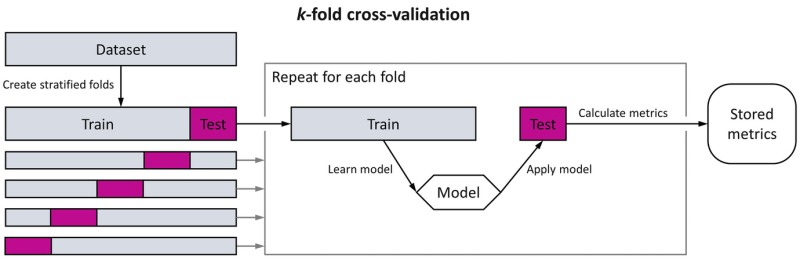
\includegraphics[width=\textwidth]{k-fold-cv}
  \caption{5-fold cross-validation (from Kubben et al \fcite{kubben2019fundamentals}}
  \label{fig:k-fold-cv}
\end{figure}

K-fold cross validation has been extended to repeat the entire experiment. A common variation is 10 times 10-fold cross-validation in which we split the data into 10 partitions, used each combination of 9 folds to train the data with the remaining partition to calculate the test error. This random splitting into 10 partitions is repeated 10 times and the 10-fold cross-validation carried out for each repetition. The 100 calculated test errors are then averaged (or summed) to give the mean (or total) error for the given hyperparameters.

A special case of k-fold CV is leave-one-out cross-validation (LOOCV) in which $k=n$, where $n$ is the number of observations. LOOCV generally results in low variance in the calculated test errors as there is less variation between the training sets than if the more data is left for the test set.

Generalized cross validation (GCV) was introduced by Craven and Wahba \fcite{craven1978smoothing}. It is a modification of LOOCV which I will not explain fully here, but know that it is commonly used in simulation studies, e.g. Fan and Li \fcite{fan2002variable}, and Hunter and Li \fcite{hunter2005variable}.

\subsubsection{Minimum Description Length}\label{sec:mdl}

Minimum description length (MDL) is a model selection principle at its core. Sometimes referred to as a formalization of Occam's Razor, it can be defined as follows:

\begin{definition}[Minimum Description Length]\label{def:mdl}
The model which can best describe the data with the least information stored about the model itself should be selected.
\end{definition}

The MDL is not an algorithm or a method in itself, but a principle which is applicable and followed in many settings. For a thorough look at MDL, I refer the reader to Grunwald \fcite{grunwald2007minimum}. Think about what the description length is: information must be stored to describe the model and the data. The more information we store about the model, the lower the cost of describing the data and vice versa. This can be likened to the bias-variance tradeoff.

\section{Penalized Likelihood Methods}

In theory, one could find a suitable estimate to the parameter vector $\Beta$ by finding the MLE as given by \cref{mle}. This rarely gives the best model as the estimate tends to describe the observed data very well but is lacking in predictive power when applied to new results due to overfitting.

A common technique used to make the model more interpretable is called regularisation. Formally, regularisation is defined as the process of adding information to an ill-posed optimisation problem to prevent overfitting. In the context of this thesis, regularisation is synonymous with penalization of a loss function.

The AIC and BIC mentioned above are actually penalized likelihood methods and could theoretically be used in the same way as the methods I will talk about below. This is generally not a preferred method though.

\begin{definition}[Loss Function]
A function which gives a curve of loss in optimisation problems.
\end{definition}

Some commonly used loss functions are 

\begin{itemize}
    \item Mean Squared Error,
    \item Mean Squared Logarithmic Error,
    \item Mean Absolute Error,
    \item Hinge Loss, and
    \item Kullback-Leibler Divergence Loss.
\end{itemize}

This is by no means an exhaustive list and in fact the methods discussed below do not use any of these loss functions.

The standard approach taken when dealing with censored survival analysis is to regularise the negative log-likelihood function by adding a penalty function. The form of this penalty varies by method and I will discuss some of the popular penalties below. A desirable feature of the penalty function is convexity; if the penalty function is convex, the minimisation of the penalised loss function become a convex optimisation problem for which there are many very efficient solutions.

Note that it need not be the exact log-likelihood used in the loss function, more often than not either the Breslow or Efron approximation to the likelihood function is used.

It can be seen that using various penalties in the loss function, ie. adding them to the MLE, is basically equivalent to assuming some prior distribution in the MAP. This prior distribution or penalty can be selected based on prior knowledge or desired features of the model, e.g. sparsity.

Fan and Li \fcite{fan2001variable} proposed a general form of a penalized likelihood function. Similar to this form but adapted slightly to the notation used here, a general form of the penalised likelihood function is

\begin{equation}\label{eqn:general-penalised-likelihood}
    l(\Beta;\x)-\lambda\sum_{j=1}^pg(|\beta_j|),
\end{equation}

where $g(\cdot)$ is a penalty function and $\lambda$ is the tuning parameter.

Different penalty functions obviously penalise the likelihood in different ways, resulting in different methods that can be used and different features of the estimator which will result.

\subsection{Hyperparameter Estimation}

The problem of model selection can very often be decomposed into a problem of parameter selection (those within the model) and hyper-parameter estimation (those outside of the model). The hyperparameters are those which are not involved in the likelihood itself, but are instead tuning parameters in the method to find the best estimate. The hyperparameters can be found using the same methods discussed in \cref{sec:model-comparison} and from most studies, it seems that cross validation is the most popular method by which to find the optimal tuning parameters. 

Roy and Chakraborty \fcite{roy2017selection} suggested Empirical Bayes as a method for selecting hyperparamters. The advantage of using Bayesian methods for selecting hypermarameters is they are informed methods, i.e. they remember previous evaluations and use this in the calculation of future estimates. This can save a lot of computational resources at the risk of adding bias if not handled with care. See \cref{sec:bias-variance} for more information.

Some other methods such as grid search and random search can also be used, but again these are a frequentist approach and are uninformed. There are many other methods which I will not discuss here, but this gives an idea of some of the most popular methods and their utility.

Friedman et al \fcite{friedman2010regularization} and Hastie et al \fcite{hastie2009elements} both explain a fairly standard practice called the one-standard-error or one-standard-deviation rule, although the rule dates back at least to the derivation by Breiman et al \fcite{breiman1984classification}. Put simply, once the value of the tuning parameter is found that minimises the penalised likelihood function, $\lambda_{\min}$, it is generally seen to overfit the model. To counteract this, the most parsimonious model with an error within one-standard-error from $\lambda_{\min}$ is chosen. Oftentimes, this is simply the model given by $\lambda_{\min}+1\textrm{s.d.}$ as this gives the highest value of $\lambda$ within one-standard-deviation, thus penalising the model more harshly for including parameters and hopefully giving a more interpretable and accurate model. This value of the hyperparameter is referred to as $\lambda_{1se}$.

\subsection{Norms}

\begin{definition}[Norm]\label{def:norm}
A norm in mathematics is a distance function which:
\begin{spacing}{0}
\begin{enumerate}
    \item commutes with scaling;
    \item obeys the triangle inequality; and
    \item is zero only at the origin.
\end{enumerate}
\end{spacing}
\end{definition}

The most common and well-known norms belong to the Minkowski family of distances given by

\begin{equation}
    \Vert\Beta\Vert_\p = \bigg(\sum_{j=1}^p|\beta_j|^\p\bigg)^{\frac{1}{\p}}.
\end{equation}

The following are some special cases of the Minkowski distance:

\begin{definition}[$L_1$-norm | Manhattan Distance]\label{def:manhattan-distance}
\begin{equation}\label{eqn:manhattan-distance}
    \Vert\Beta\Vert_1 = \sum_{j=1}^p|\beta_j|,
\end{equation}
\end{definition}

\begin{definition}[$L_2$-norm | Euclidean Distance]\label{def:euclidean-distance}
\begin{equation}\label{eqn:euclidean-distance}
    \Vert\Beta\Vert_2 = \bigg(\sum_{j=1}^p|\beta_j|^2\bigg)^{\frac{1}{2}}.
\end{equation}
\end{definition}

There is some confusion in literature attributed to an abuse of notation when speaking about the $L_0$-norm. Typically, especially in the context of variable selection and penalized likelihood, when the $L_0$-"norm" is mentioned, the author is referring to

\begin{equation}
    \Vert\Beta\Vert_0 =\sum_{j=1}^p|\beta_j|^0,\;\;\textrm{where}\;\;0^0=0.
\end{equation}

Therefore the $L_0$-"norm" (which I will henceforth be referring to as the $L_0$-norm is) counts the number of non-zero distances. It is not a norm at all because by \cref{def:norm} it is clear that it does not commute with scaling, i.e. it doesn't matter how large the distance in a given direction is as long as it is not zero.

These norms have been suggested as penalty functions in the standard form of the penalised likelihood function given by \cref{eqn:general-penalised-likelihood}. These penalties correspond to the penalised likelihood methods below.

\subsubsection{Best Subset Regression}

Best subset selection is an old statistical technique dating back at least to the introduction by Beale et al. \fcite{beale1967discarding}, and Hocking and Leslie \fcite{hocking1967selection}. Best subset regression quite literally aims to find the best subset of $q$ variables to include in the final model.

According to Wen et al \fcite{wen2017bess}, in constrained form, the problem can be written as

\begin{equation}
    \hat\Beta^{BESS}=\argmin_{\Beta} -l(\Beta;\x)\;\;\textrm{subject to}\;\;\Vert\Beta\Vert_0=q,
\end{equation}

where $l(\Beta;\x)$ is the appropriate log-likelihood or approximation mentioned in \cref{sec:partial-likelihood}. In penalised form\footnote{Tibshirani \fcite{tibshirani2016closer} stated that these problems are not equivalent.}, the problem is given by

\begin{equation}
    \hat\Beta^{BESS} = \argmin_{\Beta}\Big(-l(\Beta;\x)+\lambda\sum_{j=1}^p\Vert\beta_j\Vert_0\Big).
\end{equation}

An interesting development by Bertsimas et al \fcite{bertsimas2016best} was that best subset regression has a Mixed Integer Optimisation (MIO) formulation. This means the number of covariates that can be used with best subset regression has been hugely increased due to the extreme efficiency of MIO algorithms. I will not go into more detail about MIO here, but I direct the reader to Hastie et al \fcite{hastie2017extended} for a discussion about the effects this has and how it has changed the usage of the method.

\subsubsection{LASSO Regression}\label{sec:LASSO}

The Least Absolute Shrinkage and Selection Operator was first proposed by Tibshirani \fcite{tibshirani1996regression} for generalized linear models based on the work of Breiman \fcite{breiman1993better} with the nonnegative garotte. It was then adapted for use with the Cox PH model by Tibshirani \fcite{tibshirani1997lasso}. The two forms of the problem are given by

\begin{align}
    \hat\Beta^{lasso} =\argmin_{\Beta} -l(\Beta;\x)\;\;\textrm{subject to}\;\;\Vert\Beta\Vert_1\leq t,\\
    \hat\Beta^{lasso} = \argmin_{\Beta}\Big(-l(\Beta;\x)+\lambda\sum_{j=1}^p\Vert\beta_j\Vert_1\Big).
\end{align}

The LASSO, as the name implies, simultaneously applies shrinkage to it's included covariates, whilst promoting sparse solutions by efficiently shrinking coefficients all the way to zero. Considering its penalty term $\Vert\Beta\Vert_1$, this norm is uniquely convex while producing sparse solutions. This is because sparsity requires $p\leq1$ for $\Vert\Beta\Vert_p$ and convexity requires $p\geq1$ for $\Vert\Beta\Vert_p$. Therefore best subset regression is sparse but not convex, and ridge regression (below) is convex but not sparse.

\subsubsection{Ridge Regression}

The $L_2$-norm penalty for ridge regression is usually attributed to Hoerl and Kennard \fcite{hoerl1970ridge}. The two forms of the problem are given by

\begin{align}
    \hat\Beta^{ridge} =\argmin_{\Beta} -l(\Beta;\x)\;\;\textrm{subject to}\;\;\Vert\Beta\Vert_2^2\leq t,\label{eqn:ridge-contstrained}\\
    \hat\Beta^{ridge} = \argmin_{\Beta}\Big(-l(\Beta;\x)+\lambda\sum_{j=1}^p\Vert\beta_j\Vert_2^2\Big)\label{eqn:ridge-penalised}.
\end{align}

As with the LASSO, the two problems are equivalent because of the convexity of the problem, i.e. for any $t\geq 0$ and solution $\hat\Beta^{ridge}$ in \cref{eqn:ridge-contstrained}, there is a value of $\lambda\geq0$ such that $\hat\Beta^{ridge}$ also solves \cref{eqn:ridge-penalised}.

%SOURCE: add source for predictive accuracy studies and the overfitting caused by large coefficients
Ridge regression has been seen in multiple studies to be very accurate in prediction. It tackles the problem overfitting by shrinking the coefficients towards zero. The models produced are generally hard to interpret if the number of measured covariates is high because the coefficients are never shrunken to exactly zero.

Consider the ridge and lasso penalties. They can be visualised as follows:

\begin{figure}[h!]
  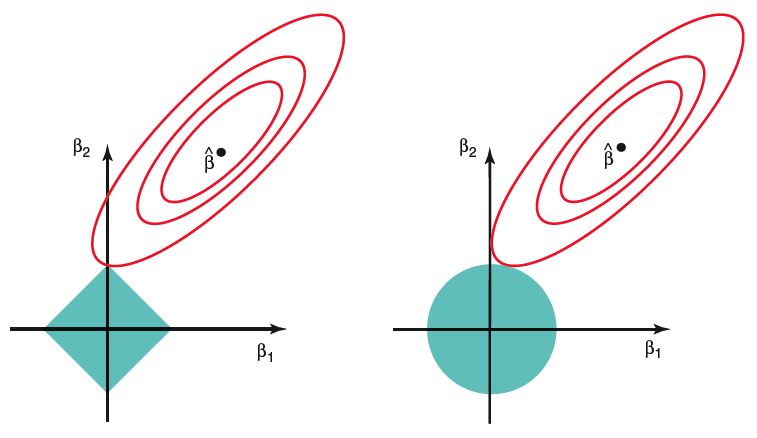
\includegraphics[width=\textwidth]{lasso-ridge}
  \caption{Estimation picture for the LASSO (left) and ridge regression(right) (from Hastie et al \fcite{hastie2009elements}}
  \label{fig:lasso-ridge}
\end{figure}

\Cref{fig:lasso-ridge} is a redrawing of a diagram dating back to Tibshirani \fcite{tibshirani1996regression}. The contours show the error and constraint functions and the shaded areas show the regions represented by the $L_1$-norm and $L_2$-norm respectively. On the left $|\beta_1|+|\beta_2|\leq t$ and on the right $\beta_1^2+\beta_2^2\leq t^2$. It can be seen in the diagram that the LASSO intercepts the constraint function along the $\beta_2$ axis, whereas the ridge regression intercepts the same contour at some positive value of both $\beta_1$ and $\beta_2$. This follows the explanation that the LASSO promotes a sparse solution as the estimator $\hat\Beta^{lasso}$ will have $\beta_1=0$ in this case. Thinking intuitively about the norm functions and their corresponding shapes given in \cref{fig:unit-circles}, it is obvious why $p\leq 1$ is a requirement to produce sparse solutions.

\begin{figure}[h!]
  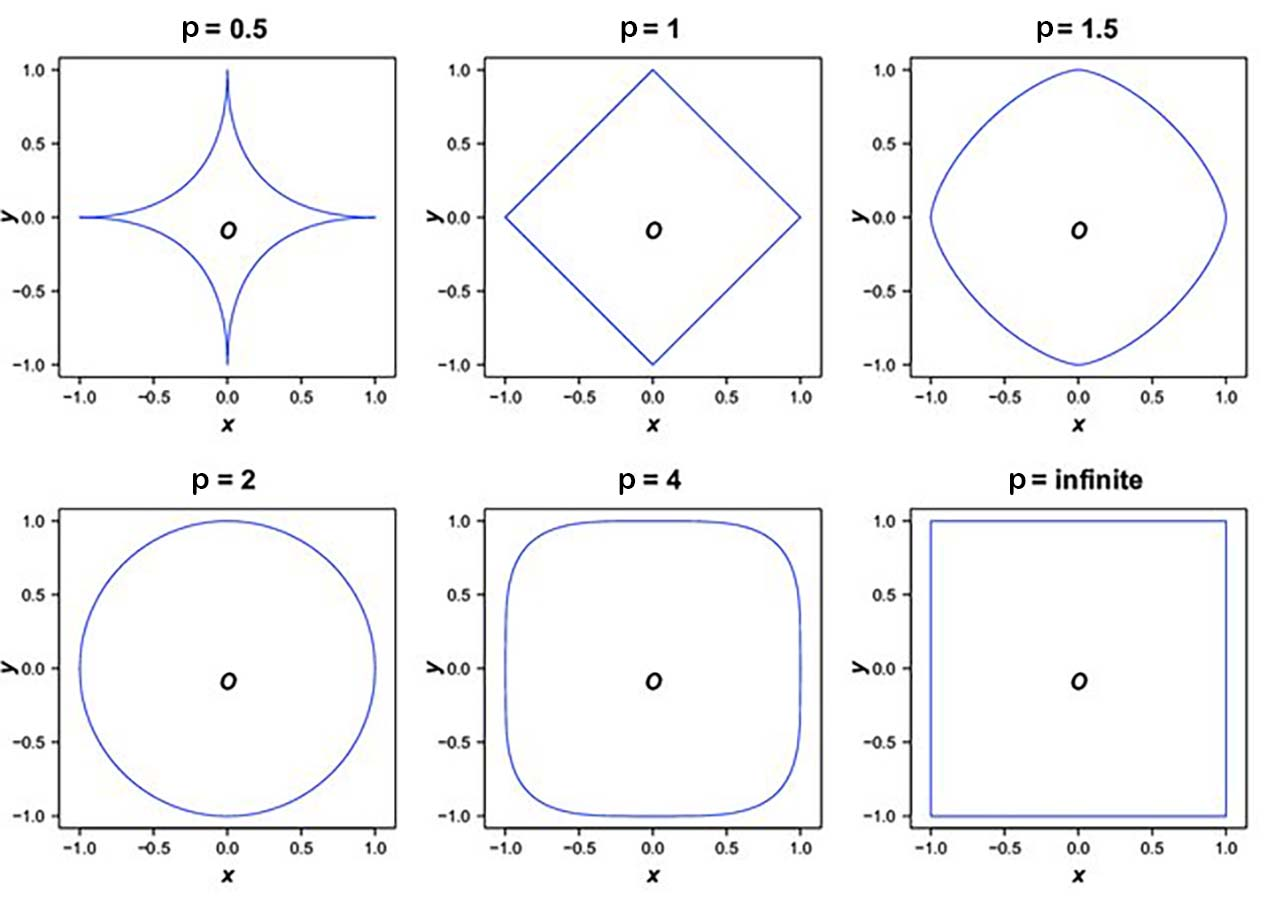
\includegraphics[width=\textwidth]{unit-circles}
  \caption{Unit circles of the Minkowski Distance in 2d with varying $p$ (from Urquiza et al \fcite{urquiza2015empirical}}
  \label{fig:unit-circles}
\end{figure}

\subsection{Bayesian Priors}
\subsubsection{Non-local priors}
Fan li 2002 [5]
\subsubsection{Shrinkage Priors}
%The Bayesian Lasso
\subsubsection{Selection Priors}
\subsubsection{Grouping Priors}
\subsubsection{Jeffrey's Priors}
\subsubsection{g-priors}
\subsubsection{Mixture Priors}
\subsection{More Frequentist Penalties}
\subsubsection{Elastic Net}

%add ref to sou and hastie 2005
The elastic net penalty is a convex combination of the $L_1$-norm and $L_2$-norm penalties proposed by Zou and Hastie \fcite{}. They showed that it had a grouping effect, meaning strongly correlated covariates tended to be included or excluded together. It is said to be very useful when $p\gg n$ and generally outperforms the LASSO while still promoting sparsity. In this paper Zou and Hastie \fcite{} also proposed an algorithm LARS-EN as an efficient computation method of the elastic net regularization pathways. Zou and Hastie \fcite{} produced \textbf{elasticnet} as an R package implementation of their method.

Friedman et al \fcite{friedman2010regularization} developed the method for the generalized linear model and proposed using cyclic coordinate descent computed along the regularization path. They produced \textbf{glmnet} as an R package implementation of the elastic net penalty for generalized linear models using coordinate descent.

Simon et al \fcite{} then introduced the method to the Cox model, again using cyclic coordinate descent and warm starts to find the solution. They showed that their method of cyclic coordinate descent was faster than the Newton-Raphson method or Lars-like algorthms used by others. Friedman et al \fcite{} gave an update of the \textbf{glmnet} package to include the new algorithm \emph{coxnet} by Simon et al \fcite{}

The actual penalty function of the elastic net for the cox model is given by

\begin{equation}
    \lambda P_\alpha(\Beta) = \lambda\Big(\alpha\sum_{j=1}^p|\beta_j|+\frac{1}{2}(1-\alpha)\sum_{j=1}^p|\beta_j|^2\Big)
\end{equation}

This gives the two forms of the optimisation problem as

\begin{align}
    \hat\Beta^{net}(\lambda,\alpha) = \argmin_{\Beta} -l(\Beta;\x)\;\;\textrm{subject to}\;\;\alpha\sum_{j=1}^p|\beta_j|+\frac{1}{2}(1-\alpha)\sum_{j=1}^p|\beta_j|^2\leq t,\label{eqn:net-contstrained}\\
    \hat\Beta^{net}(\lambda,\alpha)=\argmin_{\Beta}\Big(-l(\Beta;\x)+\lambda\bigg[(\alpha\sum_{j=1}^p|\beta_j|+\frac{1}{2}(1-\alpha)\sum_{j=1}^p|\beta_j|^2\bigg]\Big)\label{eqn:net-penalised}.
\end{align}

Consider the constraint in \cref{eqn:net-contstrained} for a moment. Based off the unit circles in \cref{fig:unit-circles}, the shape of the elastic net must be some convex combination of $p=1$ and $p=2$, and so the contour of the elastic net penalty will always lie between the diamond shape of the LASSO and the circle shape of the ridge regression.

It is worth noting that the elastic net has LASSO and ridge regression both as special cases: LASSO is achieved when $\alpha=1$; ridge regression is achieved when $\alpha=0$. This means with with just \textbf{glmnet}, LASSO, ridge regression and a convex combination of the two can be analysed.

\subsubsection{Relaxed LASSO}

The relaxed LASSO was first proposed by Meinshausen \fcite{meinshausen2007relaxed} and then simplified by Hastie et al \fcite{hastie2017extended}. I will define it similarly to them here. Let $\hat\Beta^{lasso}(\lambda)$ be the lasso estimator for the give $\lambda$. Let $A_\lambda$ be the active set - the set of all included covariates - and $\hat\Beta_{A_\lambda}^LS$ be the least squares coefficients by fitting $T$ on $\Z_{A_\lambda}$, where $T$ is the set $\{t_i\forall i=1,\ldots n\}$ and $\Z_{A_\lambda}$ is the submatrix of set of all covariate vectors with only the $A_\lambda$ active covariates. Now let $\hat\Beta^{LS}(\lambda)$ be the $p$-dimensional version, i.e. every covariate is included padded appropriately with zeros. The relaxed LASSO estimator is then given by

\begin{equation}
    \hat\Beta^{relax}(\lambda,\gamma)=\gamma\hat\Beta^{lasso}(\lambda)+(1-\gamma)\hat\Beta^{LS}(\lambda),
\end{equation}

with hyperparameters $\lambda\geq0$ and $\gamma\in[0,1]$.

I will not go into more detail here on the workings and properties of the relaxed LASSO, but know it has been found by Hastie et al \fcite{hastie2017extended} that the relaxed LASSO performs as well as LASSO in its preferred low SNR scenarios and performs as well as best subset selection in its preferred high SNR scenarios.

\subsubsection{SCAD}

\subsubsection{Adaptive LASSO}
adaptive lasso and it's oracle properties
\subsubsection{Adaptive Elastic Net}
%Zou & Zhang 2009
\subsubsection{Spike-and-Slab LASSO}
\subsubsection{Group LASSO}
%Meier et al 2008

\subsubsection{Sparse-Group LASSO}
\subsubsection{HARD}

\subsubsection{Local Quadratic Approximation}
%Fan & Li 2001
\subsubsection{Minorization-Maximisation}
%Hunter & Li 2005 VARIABLE SELECTION USING MM ALGORITHMS
\subsubsection{Firth's Penalised Likelihood}
%http://finzi.psych.upenn.edu/library/coxphf/html/coxphf.html

\section{Resampling}
%https://benthamopen.com/FULLTEXT/TOPHJ-12-136
\subsection{Jackknife}
\subsection{Bootstrapping}

\section{Ensemble Learning Methods}
%https://en.wikipedia.org/wiki/Ensemble_learning
%https://reader.elsevier.com/reader/sd/pii/S001048252100038X?token=33FFE1A8567973E72DE5114384E6E21F7B8428BD76771F533C17B3F8801616E60E22FE55694095D76A103BEC24190626&originRegion=eu-west-1&originCreation=20210419113204
%https://machinelearningmastery.com/bagging-and-random-forest-ensemble-algorithms-for-machine-learning/#:~:text=Bootstrap%20Aggregation%20(or%20Bagging%20for,predictions%20than%20any%20individual%20model.
%https://www.tandfonline.com/doi/full/10.1080/21642583.2019.1620658
SVR
VSEs
Weak Learner
Strong Learner
\subsection{Boosting}
%https://www.hindawi.com/journals/cmmm/2013/873595/
%https://towardsdatascience.com/boosting-algorithms-explained-d38f56ef3f30
\subsection{Model-Based Boosting}
\subsection{Likelihood-Based Boosting}
\subsection{Bagging}
\subsection{Stacking}
\subsection{Bayes Optimal Classifier}
\subsection{Bayesian Model Averaging}
%Bayesian Structure Time Series
\subsection{Bayesian Model Combination}
\subsection{Bucket of Models}
\subsection{Stability Selection}
%https://www.hindawi.com/journals/cin/2017/2747431/

\section{Regularization Paths}

If a model has at most $p$ covariates, then a regularization path is a path in a $p$-dimensional space. The path is determined by the value of all the coefficients for a given value of the hyperparameter vector $\THETA$. The regularized function, i.e. the maximum penalised partial likelihood function in the case of Cox PH regression, determines the rough shape of the regularization pathways. However, different algorithms will differ slightly; some are continuous, some are piece wise continuous, et cetera. The efficiency of calculation of the regularization path, generally determines the computational cost of the method.

I will not go into detail on the theory or background of regularization paths here, as generally speaking the variable selection methods I will be testing in the simulation studies will already have selected their chosen technique of path calculation. I will however explain some of the popular algorithms I have mentioned above as they play a substantial role in computation time which can be a determining factor in when a particular method can be used.

\subsection{Newton-Raphson}

\subsection{LARS}
%https://en.wikipedia.org/wiki/Least-angle_regression
%http://finzi.psych.upenn.edu/library/covTest/html/lars.glm.html

\subsubsection{LARS-EN}

\subsection{Coordinate Descent}

\subsection{Forward Stepwise Regression}

Forward Stepwise and Forward Stagewise regression are old techniques typically attributed to Efryomson \fcite{efroymson1966stepwise}, and Draper and Smith \fcite{draper1966applied}. Efron et al \fcite{efron2004least} then brought the methods back to the forefront upon deriving a connection between forward stagewise estimates and the solution path to the LASSO\ucite{tibshirani2015general} which I spoke about in \cref{sec:LASSO}. The algorithm is given concisely by Tibshirani \fcite{tibshirani2015general}:

\begin{algorithm}[H]
    Fix $\epsilon>0$\;
    Initialise $\Beta^{(0)}=0$\;
    \For{$k=1,2,\ldots$}{
    $\Beta^{(k)}=\Beta^{(k-1)}+\epsilon\cdot\textrm{sign}(\z_i^T(t-\z\Beta^{(k-1)}))\cdot e_i$, where $i\in\argmax_{j=1,\ldots,p}|\z_i^T(t-\z\Beta^{(k-1)})|.$
    }
    \caption{Forward stagewise regression (from Tibshirani \fcite{tibshirani2015general})}\label{alg:forward-stagewise-regression}
\end{algorithm}

Following the results of Bertsimas et al \fcite{bertsimas2016best}, Hastie et al \fcite{hastie2017extended} conducted a thorough comparison of the forward stepwise regression, best subset selection and the LASSO. They summarised their findings as follows:

\begin{itemize}
    \item best subset selection generally outperforms lasso when SNR is high, conversely the opposite is true when SNR is low; 
    \item best subset selection and forward stepwise perform quite similarly throughout;
    \item relaxed LASSO performed similarly to the optimal methods at high and low SNR and was dubbed the overall winner.
\end{itemize}

\section{More Selection Methods}

\subsection{Heirarchical Bayesian Method} 
%https://pubmed.ncbi.nlm.nih.gov/9147593/

\subsection{SIS}
%Sure independence screening for ultrahigh dimensional feature space
%High-dimensional variable selection for Cox’s proportional hazards model
blessing of dimensionality 
\subsubsection{ISIS}
%Ultrahigh dimensional variable selection: beyond the linear model

\section{Hypothesis Testing}
\subsection{Likelihood-Ratio Test}
\subsection{Wald Test}
\subsection{Lagrange Multiplier (Score) Test}

\section{Extended Variable Selection Problems}
\subsection{Required Covariates}
\subsection{Missing Covariates}
\subsection{Ultrahigh Dimensionality}
\subsection{Associated / Collinear Covariates}
\subsection{Case-Cohort Studies}
%Variable selection for case-cohort studies with failure time outcome - Ni et al 2016

\part{Simulation Study}
- Convergence
- Model Stability


- BeSS
- bestsubset
- My.stepwise.coxph
- glmnet
- 

\part{Real-World Example}
